\documentclass[notes=hide,handout]{beamer}
\usetheme{Warsaw}
%\setbeamercolor{structure}{fg=cyan!90!black}
\usecolortheme{spruce}
\usepackage{beamerthemesplit}
\usepackage{amssymb,latexsym,amsmath}
\usepackage{amsthm}
\usepackage{epsfig}
\usepackage{setspace}
\usepackage{blkarray}
%\usepackage{showkeys} %shows labels for referencing in pdf. Comment out in final paper. 
%-----------------------------------------------------------------
\vfuzz2pt % Don't report over-full v-boxes if over-edge is small
\hfuzz2pt % Don't report over-full h-boxes if over-edge is small
% THEOREMS -------------------------------------------------------
\theoremstyle{plain}
\newtheorem{thm}{Theorem}[section]
\newtheorem{cor}[thm]{Corollary}
\newtheorem{lem}[thm]{Lemma}
\newtheorem{prop}{Proposition}[section]
\theoremstyle{definition}
\newtheorem{defn}[thm]{Definition}
\theoremstyle{remark}
\newtheorem{rem}{Remark}
\theoremstyle{definition} 
\newtheorem{ex}{Example}[section]
\numberwithin{equation}{section}
\newtheorem{prob}{Problem}
\numberwithin{equation}{section}
\newtheorem{eqn}{}
% MATH -----------------------------------------------------------
\newcommand{\norm}[1]{\left\Vert#1\right\Vert}
\newcommand{\abs}[1]{\left\vert#1\right\vert}
\newcommand{\set}[1]{\left\{#1\right\}}
\newcommand{\Real}{\mathbb R}
\newcommand{\Z}{\mathbb{Z}}
\newcommand{\eps}{\varepsilon}
\newcommand{\TO}{\longrightarrow}
\newcommand{\To}{\longmapsto}
\newcommand{\BX}{\mathbf{B}(X)}
\newcommand{\A}{\mathcal{A}}
\newcommand{\gen}[1]{\left\langle#1\right\rangle}
\newcommand{\mat}[2][rrrrrrrrrrrrrrrrrrrrrrrrr]{\left(\begin{array}{#1}#2\\ \end{array}\right)}
\newcommand{\iso}{\cong}
\newcommand{\semidirect}{\rtimes}
\newcommand{\all}{\text{ for all }}
\newcommand{\stab}[2]{\text{Stab}_{#1}\left(#2\right)}
\renewcommand{\ker}[1]{\text{ker}\left(#1\right)}
\newcommand{\im}[1]{\text{im}\left(#1\right)}
\newcommand{\soc}[1]{\text{Soc}\left(#1\right)}
\newcommand{\Aut}[1]{\text{Aut}\left(#1\right)}
\newcommand{\Inn}[1]{\text{Inn}\left(#1\right)}
\newcommand{\Out}[1]{\text{Out}\left(#1\right)}
\newcommand{\rank}[1]{\text{rank}\left(#1\right)}
\newcommand{\st}{\text{ such that }}
\newcommand{\simpcomp}[1]{ ^{\text{simp}}_{\text{comp}}\{#1\}}
\newcommand{\boundary}{\partial}
\newcommand{\Hom}[2]{{\ker{#1}}/{\im{#2}}}
\newcommand{\finitefield}[1]{\Z/{#1\Z}}
\renewcommand{\dim}[1]{\text{dim}\left(#1\right)}
\newcommand{\Cayley}[2]{\text{Cayley}\left(#1,#2\right)}
\renewcommand{\epsilon}{\varepsilon}
\newcommand{\twhite}[1]{\textcolor{white}{#1}}
%simplices--------------------------------------------------------
\newcommand{\vertex}[1]{\text{F}_{0}\left(#1\right)}
\newcommand{\edge}[2]{\text{F}_{1}\left(#1,#2\right)}
\newcommand{\triang}[3]{\text{F}_{2}\left(#1,#2,#3\right)}
\newcommand{\tetra}[4]{\text{F}_{3}\left(#1,#2,#3,#4\right)}
\newcommand{\nsimplex}[3]{\text{F}_{n}\left(#1,#2,...,#3\right)}

% ----------------------------------------------------------------
%footnotes with symbols
\long\def\symbolfootnote[#1]#2{\begingroup%
\def\thefootnote{\fnsymbol{footnote}}\footnote[#1]{#2}\endgroup} 
% ----------------------------------------------------------------
%drawing
%\usepackage[svgnames]{xcolor}
\usepackage{tikz}
\usepackage{caption}
\usepackage{amsmath}
\usetikzlibrary{matrix,arrows,backgrounds}
\usetikzlibrary{patterns}


\pgfdeclarelayer{edgelayer}
\pgfdeclarelayer{nodelayer}
\pgfsetlayers{edgelayer,nodelayer,main}

\tikzstyle{none}=[inner sep=0pt]
\tikzstyle{rn}=[circle,fill=Red,draw=Black,line width=0.8 pt]
\tikzstyle{gn}=[circle,fill=Lime,draw=Black,line width=0.8 pt]
\tikzstyle{yn}=[circle,fill=Yellow,draw=Black,line width=0.8 pt]
\tikzstyle{black}=[circle,fill=Black,draw=Black]

%\usepackage[graphics,tightpage,active]{preview}
%\PreviewEnvironment{tikzpicture}
\newlength{\imagewidth}
\newlength{\imagescale}

\usenavigationsymbolstemplate{}
%----------------------------------------------------------------

\title[Optimal Helical Compression Springs]{Given a Helical Compression Spring in a Spring-Mass Damper System: What are Optimal Springs?}
\author[Sandia National Laboratories Group]{A. Bentley, T. Hodges, J. Jiang, J. Krueger, S. Nannapaneni, T. Qiu}
\institute[]{2015 Industrial Math/Stat Modeling Workshop for Graduate Students} 
\date{July 22, 2015}

\begin{document}

\frame{
\titlepage
}
\section{Problem}
\frame{
\frametitle{Problem}
\begin{columns}[c]
\column{.5\textwidth}
\begin{itemize}
	\item Design an algorithm that optimizes springs with interchangeable constraints and objectives.
	\item Can you quantify and incorporate stress relaxation?
	\item Incorporate design optimization uncertainty.
	
\end{itemize}
\column{.5\textwidth}
\begin{figure}[h]
		 \begin{center}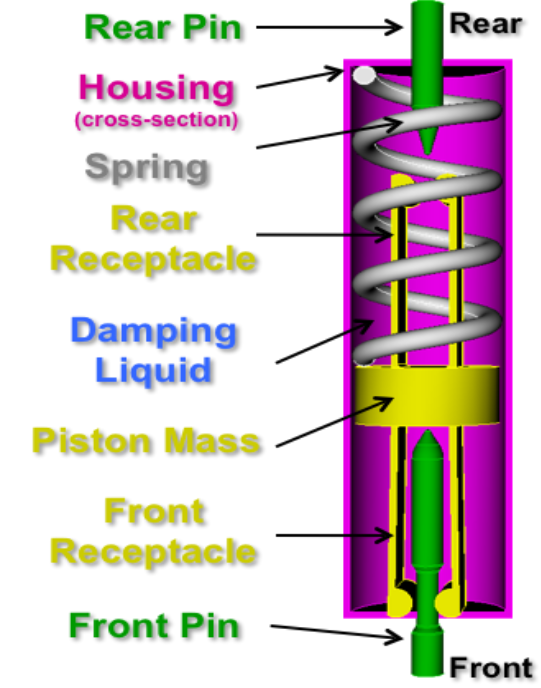
\includegraphics[scale=.2]{Acceleration_Switch_Detailed.png}\end{center}
		 \caption{Acceleration switch}
		 \label{fig:Acceleration_Switch}
		 
		 \end{figure}	 
\end{columns}
}

\section{Approach}
\frame{
\frametitle{Algorithm}
\begin{columns}[c]
\column{.5\textwidth}
\begin{itemize}
	\item What do we need in include in the algorithm? 
	\item Feasibility, Sensitivity Analysis, Optimization. 

	
\end{itemize}
\column{.5\textwidth}
\begin{figure}[h]
		 \begin{center}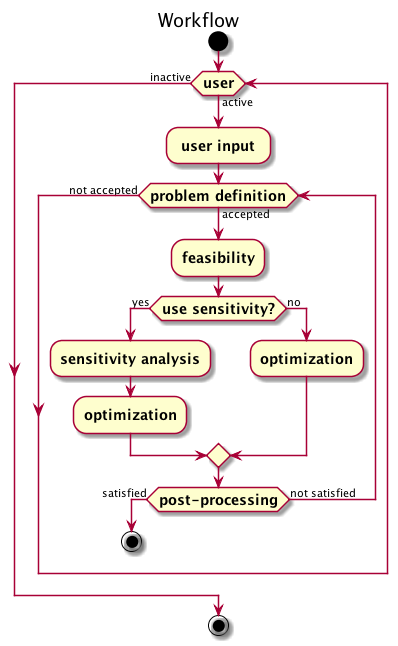
\includegraphics[scale=.28]{IMSM_Workflow.png}\end{center}
		 \caption{Algorithm of approach}

		 
		 \end{figure}	 
\end{columns}
}

\frame{
\frametitle{User Input}
\begin{columns}[c]
	\column{.5\textwidth}
\begin{figure}[h]
		 \begin{center}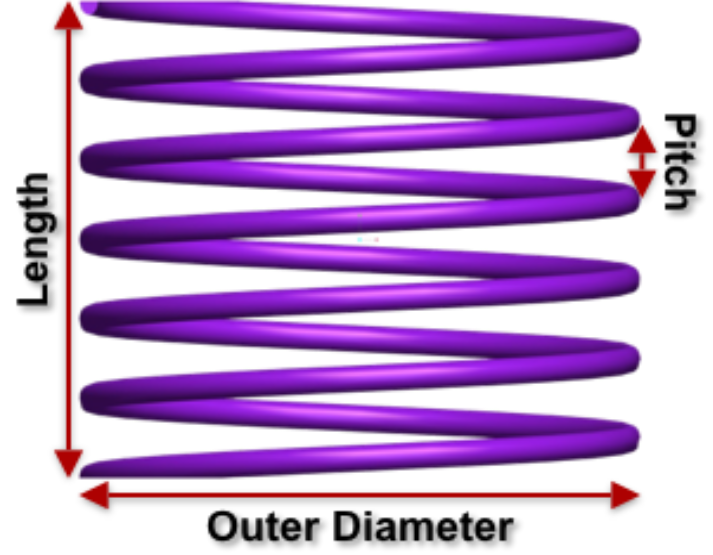
\includegraphics[scale=.1]{Spring_Description.png}\end{center}
		 \caption{Outer diameter, pitch, and \\free length.}
		 \label{fig:Description1}
\end{figure}	

\begin{figure}[h]
		 \begin{center}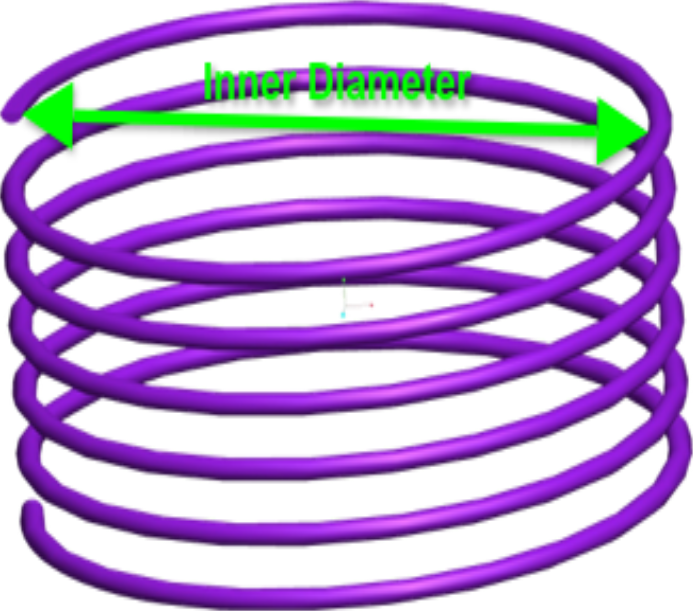
\includegraphics[scale=.1]{Spring_Description2.png}\end{center}
		 \caption{Inner diameter}
		 \label{fig:Description2}
\end{figure}
	
	\column{.5\textwidth}
	\begin{figure}[h]
		 \begin{center}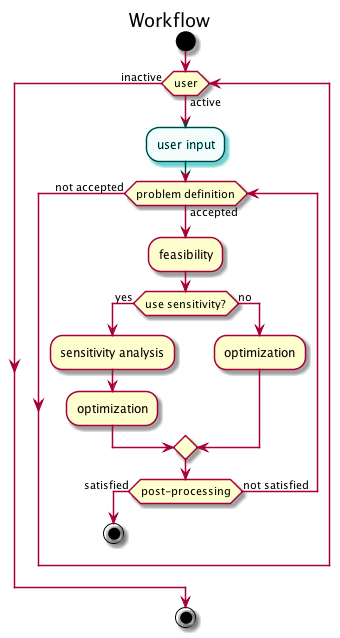
\includegraphics[scale=.28]{IMSM_Workflow1.png}\end{center}
		 \caption{User Input}

		 
		 \end{figure}
	

	 
\end{columns}


}

\frame{
\frametitle{Problem Definition}
\begin{columns}[c]
	\column{.5\textwidth}
				\begin{equation*}
 					\begin{aligned}
 						& \underset{\textbf{x}}{\text{min}}
 						& & F(\textbf{x}), \\
 						& \text{subject to}
 						& & G(\textbf{x}) \le 0
 					\end{aligned}
				\end{equation*}



	
	\column{.5\textwidth}
	\begin{figure}[h]
		 \begin{center}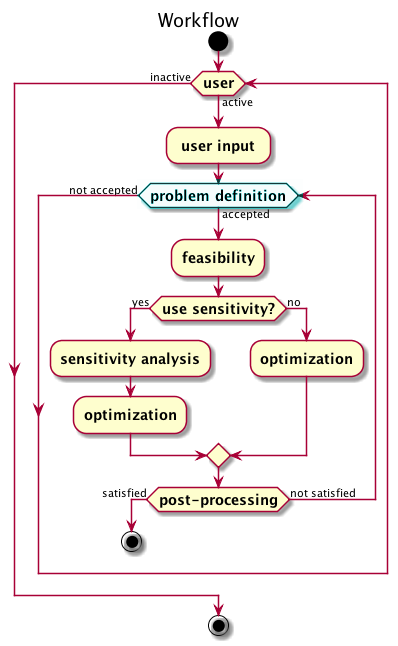
\includegraphics[scale=.28]{IMSM_Workflow2.png}\end{center}
		 \caption{Problem Definition}
	
		 
		 \end{figure}
	

	 
\end{columns}


}


\frame{
\frametitle{Feasibility}
\begin{columns}[c]
\column{.5\textwidth}
\begin{figure}[h]
		 \begin{center}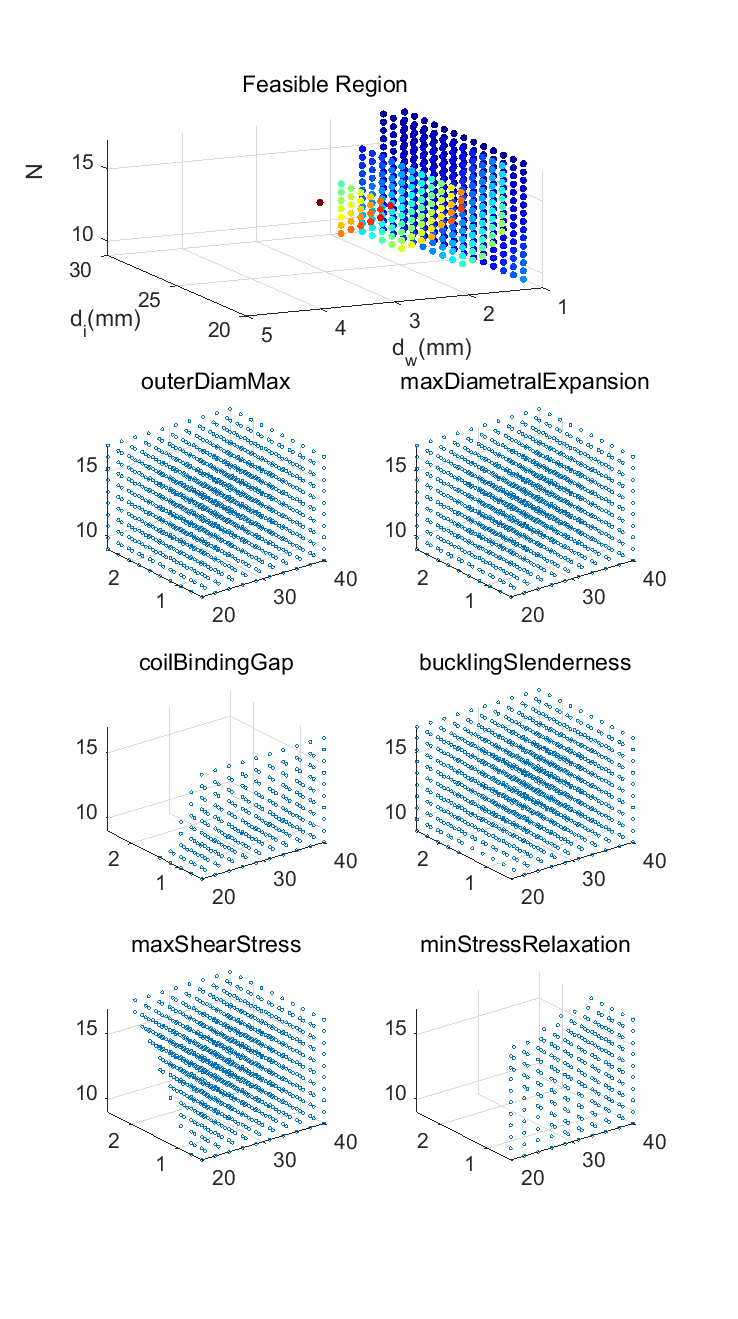
\includegraphics[scale=.28]{Case_56_38910new.eps}\end{center}
		 \caption{Feasibility Region}
		 \label{fig:Region2}
\end{figure}	
\column{.5\textwidth}
	\begin{figure}[h]
		 \begin{center}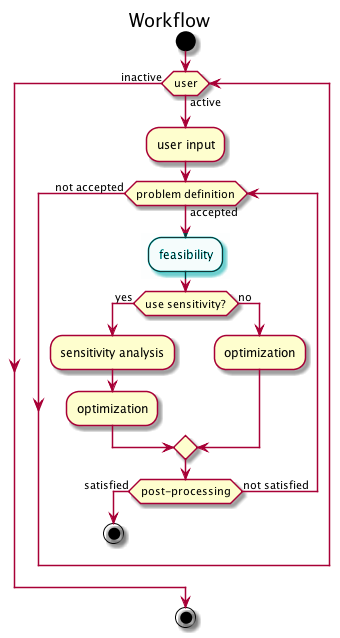
\includegraphics[scale=.28]{IMSM_Workflow3.png}\end{center}
		 \caption{Feasibility}
	
		 
		 \end{figure}


\end{columns}


}


\frame{
\frametitle{Sensitivity Analysis}
\begin{columns}[c]
	\column{.6\textwidth}
	\begin{itemize}
		\item If dim(design space) increases then computation expense increases.
		\item Sensitivity Analysis $\rightarrow$ Measure of influence
		\item Locally $\rightarrow$ around a point (Gradient).
		\item Globally $\rightarrow$ Overall sensitivity (Sobol Indices).
		\item $Y = G(X_{1},...,X_{n})$
		\item Sobol Index: $S_{i}^{I} = \frac{V_{i}(E_{~i}(Y | X_{i}))}{V(Y)}$
	\end{itemize}
	
	\column{.4\textwidth}
		\begin{figure}[h]
			 \begin{center}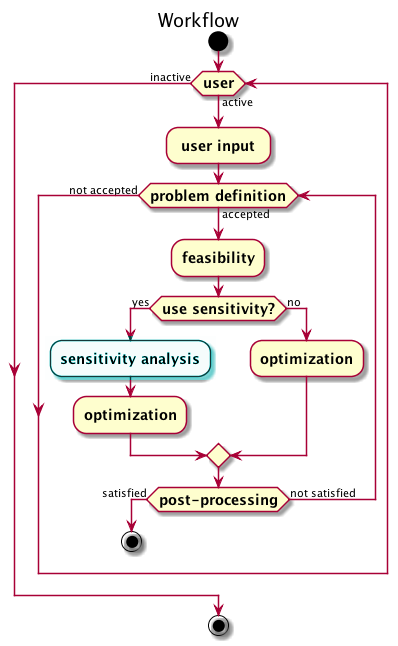
\includegraphics[scale=.28]{IMSM_Workflow4.png}\end{center}
			 \caption{Sensitivity}
	
		 
		 \end{figure}
	 
\end{columns}


}

\frame{
\frametitle{Optimization}
\begin{columns}[c]
	\column{.6\textwidth}
	\begin{itemize}
		\item Constrainted Optimization
	\end{itemize}
			\begin{equation*}
 					\begin{aligned}
 						& \underset{\textbf{x}}{\text{min}}
 						& & F(\textbf{x}), \\
 						& \text{subject to}
 						& & G(\textbf{x}) \le 0\\
						 & lb_{\textbf{x}} \le \textbf{x} \le ub_{\textbf{x}}\\
 					\end{aligned}
				\end{equation*}
	\begin{itemize}
		\item Local vs. Global
			\begin{itemize}
				\item Local, requires initial point, faster.
				\item Global, no initial point, slower.
				
			\end{itemize}	
		\item DIRECT algorithm for optimization
		\item Easily integrated with the framework.
	\end{itemize}
	
	\column{.4\textwidth}
	
		\begin{figure}[h]
		 \begin{center}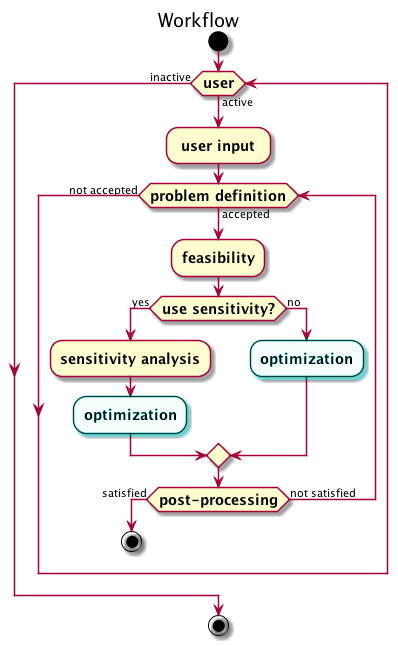
\includegraphics[scale=.28]{IMSM_Workflow5.png}\end{center}
		 \caption{Optimization}
	
		 
		 \end{figure}
	 
\end{columns}
}

\section{Stress Relaxation}
\frame{
\frametitle{Stress Relaxation}
\begin{columns}[c]
	\column{.4\textwidth}
	\begin{figure}[h]
		 \begin{center}
\includegraphics[scale=.4]{hands_revised.png}\end{center}
		
		 \end{figure}
	\column{.6\textwidth}
	\[\frac{4}{ G\theta d_w^4}\int_0^{d_w} r^2 \left( (G\theta r)^{-n} + {c\over k} Gnt^k \right)^{-\frac{1}{n}} \,\mathrm{d} r
\]
\centering where
\[
\theta = {2s\over \pi N_a ((d_i+d_o)/2)^2}
\]
	 
\end{columns}
}

\frame{
\frametitle{Design Optimization Uncertainty}

	\begin{itemize}
		\item Variability in manufacturing process $\rightarrow$ tolerance/uncertainty.
		\item Considerations in design process:
	\end{itemize}
				\begin{equation*}
 					\begin{aligned}
						& \underset{x}{\text{min}}
						  \hspace{.1in} \mu_{F}(\textbf{x},d), \\
						& \text{such that}\\
 						&  Pr(G(\textbf{x},d) <0)  > \rho_{t}\\
						&  Pr(\textbf{x} > lb_{\textbf{x}})  > \rho_{t}^{lb}\\
						&  Pr(\textbf{x} < \mu b_{\textbf{x}})  > \rho_{t}^{ub}\\
 					\end{aligned}
				\end{equation*}
		\begin{itemize}
			\item Uniform Distribution [$\mathbf{x}_{i} -  T_{\mathbf{x}_{i}}$, $\mathbf{x}_{i} +  T_{\mathbf{x}_{i}}$]
			\item Each iteration $\rightarrow$ Reliability analysis using Monte Carlo.
			\item UQ propagation with Monte Carlo to obtain $F(\mathbf{x})$
		\end{itemize}

	 

}




\frame[allowframebreaks]{
\frametitle{References}
\nocite{*}
%\cite{}
%\cite{OEIS}}\end{TINY}
%\nocite{Eisenbud}
%\nocite{DF}
%\nocite{DGPS}
%\nocite{What_Is}
%%\nocite{Greuel}
%\nocite{Maple17}
%\nocite{Mayr}
%\nocite{M2}
%\nocite{Intervals}
%\nocite{Floating}
%\nocite{Bates}
%\nocite{MATLAB:2014a}
\bibliographystyle{ieetr}
\bibliography{MyBib}
}

\frame{
\frametitle{}
\begin{center}
\LARGE Thank you.\\
\bigskip
\LARGE Questions?
\end{center}
}

\end{document}







